%%%%%%%%%%%%%%%%%%%%%%%%%%%%%%%%% Ergebnisse %%%%%%%%%%%%%%%%%%%%%%%%%%%%%%%%%%


\chapter{Ergebnisse}
\label{chap:Ergebnisse}

Die Ergebnisse, falls in Abbildungen oder Tabellen dargestellt, sollten gut lesbar sein. Zusätzlich ist das Verwenden einer Grafik als Vektorgrafik empfehlenswert, da somit eine als PDF formattierte Grafik direkt eingebettet werden kann. Das garantiert eine gute Lesbarkeit, führt jedoch nicht dazu, dass die Schriftgröße ausreichend festgelegt werden muss. Anbei befindet sich jeweils ein Beispiel für eine Grafik \ref{fig:Fig1} und eine Tabelle \ref{tab:TableExample}.


\begin{figure}[h]
  \centering
  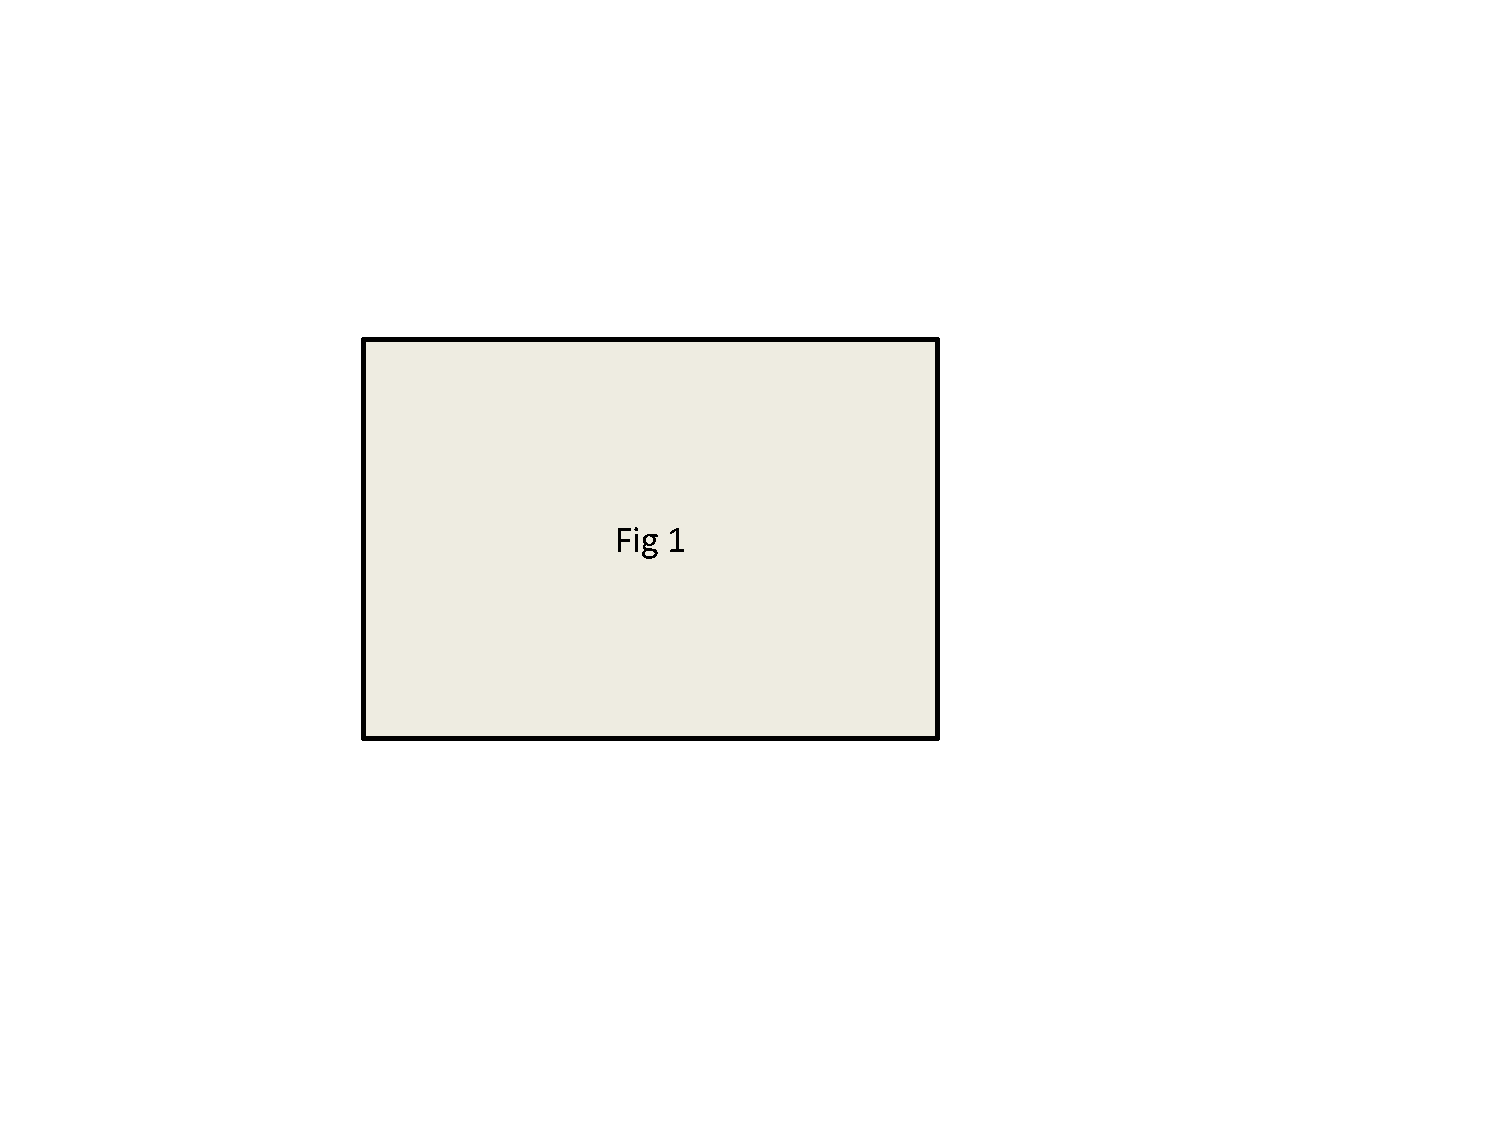
\includegraphics[width=0.95\textwidth]{Fig1.pdf}
  \caption{Beispielgrafik}
  \label{fig:Fig1}
\end{figure}

\begin{table}[!htbp]
  \centering
\resizebox{\textwidth}{!}{\begin{tabular}{|l|p{5cm}|p{5cm}|p{5cm}|}
\hline
& & &  \\
& Parameter 2	& Parameter 3	& Parameter 4 \\
& & &  \\
\hline
Datenelement 1& Datenwert 1.1& Datenwert 1.2& Datenwert 1.3 \\
Datenelement 2& Datenwert 2.1& Datenwert 2.2& Datenwert 2.3  \\
Datenelement 3& Datenwert 3.1& Datenwert 3.2& Datenwert 3.3  \\
Datenelement 4& Datenwert 4.1& Datenwert 4.2& Datenwert 4.3  \\
Datenelement 5& Datenwert 5.1& Datenwert 5.2& Datenwert 5.3  \\
\hline
\end{tabular}}
  \caption{Beispieltabelle.}
	\label{tab:TableExample}
\end{table}











%%%%%%%%%%%%%%%%%%%%%%%%%%%%%%%%% Ergebnisse %%%%%%%%%%%%%%%%%%%%%%%%%%%%%%%%%%
